\section{Implementation}
\label{sec:impl}

Our solution is designed using commodity off the shelf (COTS) components.
%
The open-source implementation\footnote{Available at: \url{https://github.com/synercys/PIRMedic}} includes:

%% BEGINNING OUTLINE
% \begin{itemize}
%     \item What features were extracted from PSD?
%     \item Compare results from PSD vs results from FFT to show that PSD is useful. 
%     \item False positives and false negatives in each fault class (correlation with working sensor) 
% \end{itemize}
%% END OF OUTLINE

\ca \textbf{Edge Hardware} consisting of -- \ci a PIR sensor~\cite{PIR_sensor_eval}, \cii a bare-metal platform~\viz Arduino Mega Microcontroller Unit (MCU)~\cite{arduino_mega} 
for sensor data capture, and \ciii a Linux-based platform~\viz Raspberry Pi~\cite{rpi3} 
for executing the fault detection and diagnosis algorithm, \sol.% as shown in {\bfseries Fig.~\ref{fig:platform_photograph}}.

% analysis (\viz feature extraction, fault classification and fault identification).

The Arduino MCU polls the sensor hardware signals (\ie \cout and \aout) periodically over a GPIO interface. We poll the PIR sensors at a frequency $\geq$ 20 Hz due to the \textit{Nyquist criterion} as the human motion information in the PIR sensor is between 0 -- 10 Hz. %Recall that the \textit{Nyquist criterion} requires that the sampling frequency be at least twice the highest frequency contained in the signal, or information about the signal will be lost while sampling. 
Note that using a bare-metal platform allows us to capture \aout samples at a constant rate. %This enables us to cleanly capture the frequency domain characteristics of the \aout signal correctly.
The Raspberry Pi platform performs the fault detection and analysis for the data captured at the Arduino MCU.
%, implemented in python. 
The Raspberry Pi and Arduino are connected via a Micro-USB cable and the data captured at the Arduino MCU is serially transferred to the Raspberry Pi for analysis. 

\cb \textbf{Edge Implementation} We used standard python libraries such as \texttt{tsfresh}~\cite{tsfresh2018code,christ2016distributed} for computing features such as FFT and other statistical features as a part pf feature extraction, \texttt{numpy} for data preprocessing and 
\texttt{xgboost}~\cite{shap_implementation} for implementing the machine learning classifiers. %Our code is available as open-source repositories\footnote{Link redacted to comply with double-blind requirements}.
The end-to-end workflow of our solution is illustrated in {\bfseries Fig.~\ref{fig:system_workflow}}.

\begin{figure}
    \begin{minipage}{0.9\textwidth}
	\centering
        %Settings for submission
	    %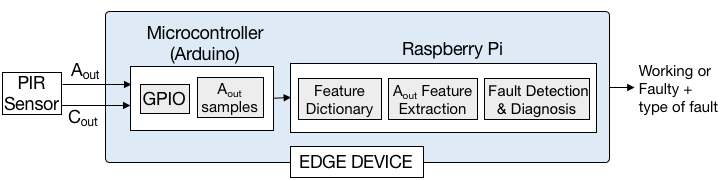
\includegraphics[width=0.5\textwidth,height=0.8in]{figures/platform/sensys_workflow-redraw-camera.png}
        %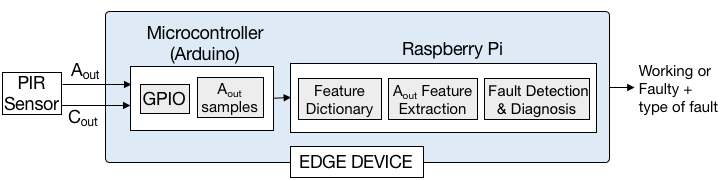
\includegraphics[width=0.5\textwidth]{figures/platform/sensys_workflow-redraw-camera.png}
        \includegraphics[width=\textwidth]{figures/platform/sensys_workflow.pdf}
    	\caption{\sol workflow for fault detection and diagnosis. The PIR sensor is connected to an Arduino microcontroller via a GPIO interface. The ADC onboard the microcontroller converts the \aout and \cout values into discrete samples that are then sent to a Raspberry Pi where the fault detection and diagnosis is performed.}
	   \label{fig:system_workflow}
    \end{minipage}
    % \hfill
    % \begin{minipage}{0.34\textwidth}
    % \centering
    % %Settings for submission
    % %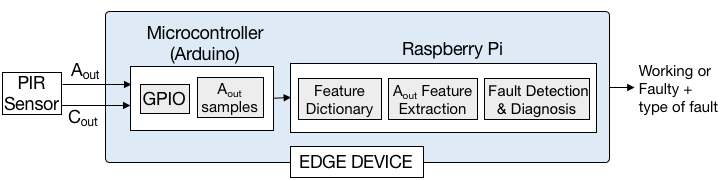
\includegraphics[width=0.5\textwidth,height=0.8in]{figures/platform/sensys_workflow-redraw-camera.png}
    % %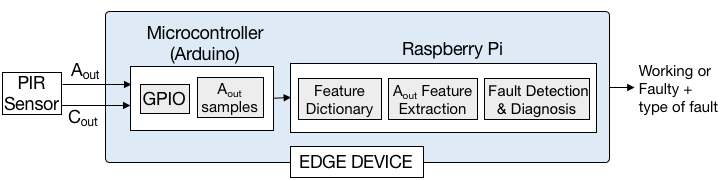
\includegraphics[width=0.5\textwidth]{figures/platform/sensys_workflow-redraw-camera.png}
    % 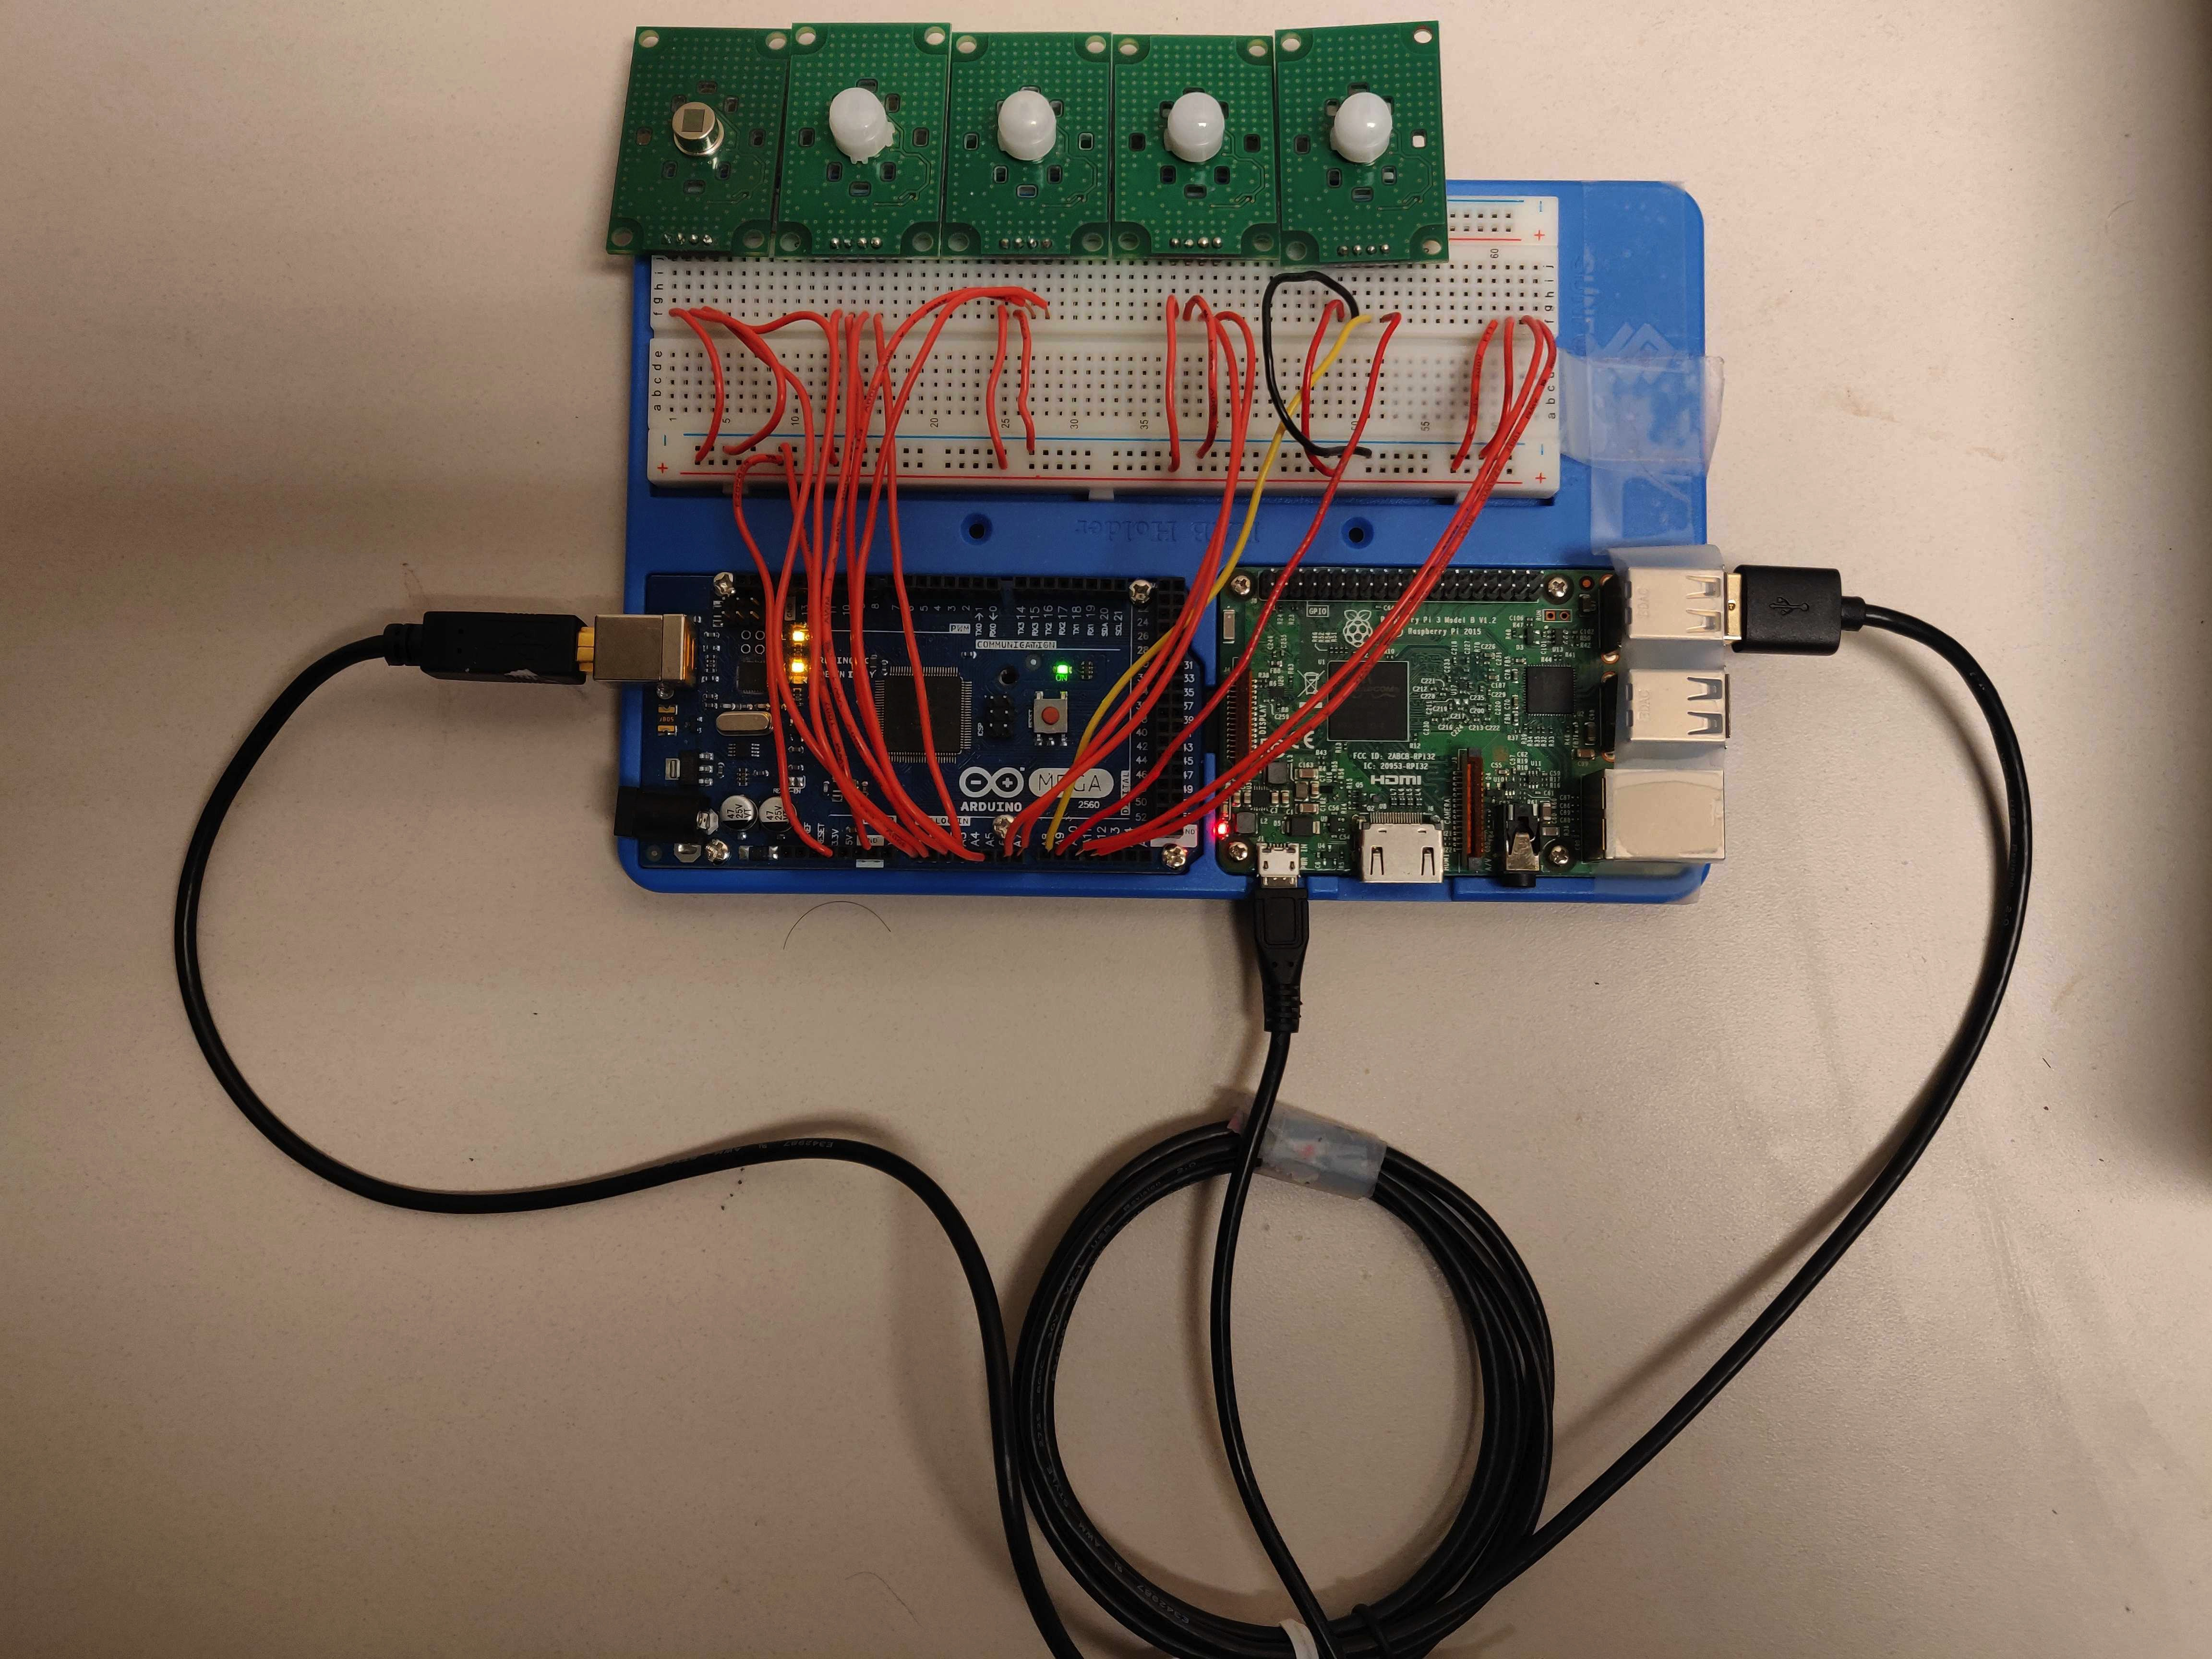
\includegraphics[width=\textwidth, height=1.2in]{figures/platform/eval_platform.jpg}
    % \caption{\ins{Evaluation Platform showing PIR sensor connected to a Raspberry Pi and Arduino Microcontroller.}}
    % \label{fig:eval_platform}
    % \end{minipage}
\end{figure}%
%
\begin{figure}
    \begin{minipage}{0.65\textwidth}
        \centering
        %\begin{table}
        %\begin{wraptable}{R}{0.65\textwidth}%[ht]\small
        %\renewcommand{\arraystretch}{1.1}
        %\vspace{-\baselineskip}
        \footnotesize
        \captionof{table}{Details of Evaluation Setup used in \sol}
        \begin{tabular}{p{2.6cm} p{6cm}}
        \hline %\\
        \textsc{\bfseries Component} & \textsc{\bfseries Specifications \& Details}\\
        \hline\hline
        \rowcolor{gray!20} \multicolumn{2}{l}{\bfseries Data Collection \& Analysis Platform}\\
        Arduino Mega 2560 Rev3 & ATmega2560 16 MHz with 256 kB Flash \\
        Raspberry Pi v3.0 Model B & Quad Core 1.2GHz Broadcom BCM2837 64bit CPU, 1GB RAM \\
        \hline
        \rowcolor{gray!20} \multicolumn{2}{l}{\bfseries Connectivity \& Power} \\
        USB Serial Cable & Interface between Raspberry Pi and Arduino Microcontroller\\
        Power Supply & 5V for Arduino and 3.3V for Raspberry Pi\\
        \hline
        \rowcolor{gray!20} \multicolumn{2}{l}{\bfseries Sensor} \\
        PIR Sensor & Murata PIR Evaluation Board IMX-060 \\
        % Thermal Faults & Pyroelectric element can degrade or age and can give imperfect output\\
        \hline
        \end{tabular}
        \label{tab:pir_platform}
        %\vspace{-15pt}
        %\vspace{-\baselineskip}
        %\end{wraptable}
        %\end{table}
    \end{minipage}
    \hfill
    \begin{minipage}{0.34\textwidth}
    	\centering
        %Settings for submission
        %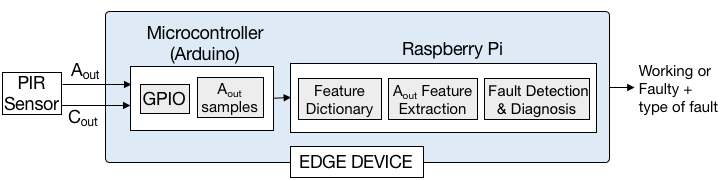
\includegraphics[width=0.5\textwidth,height=0.8in]{figures/platform/sensys_workflow-redraw-camera.png}
        %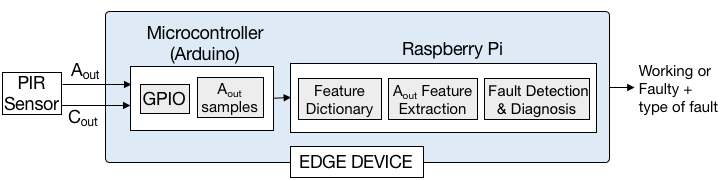
\includegraphics[width=0.5\textwidth]{figures/platform/sensys_workflow-redraw-camera.png}
        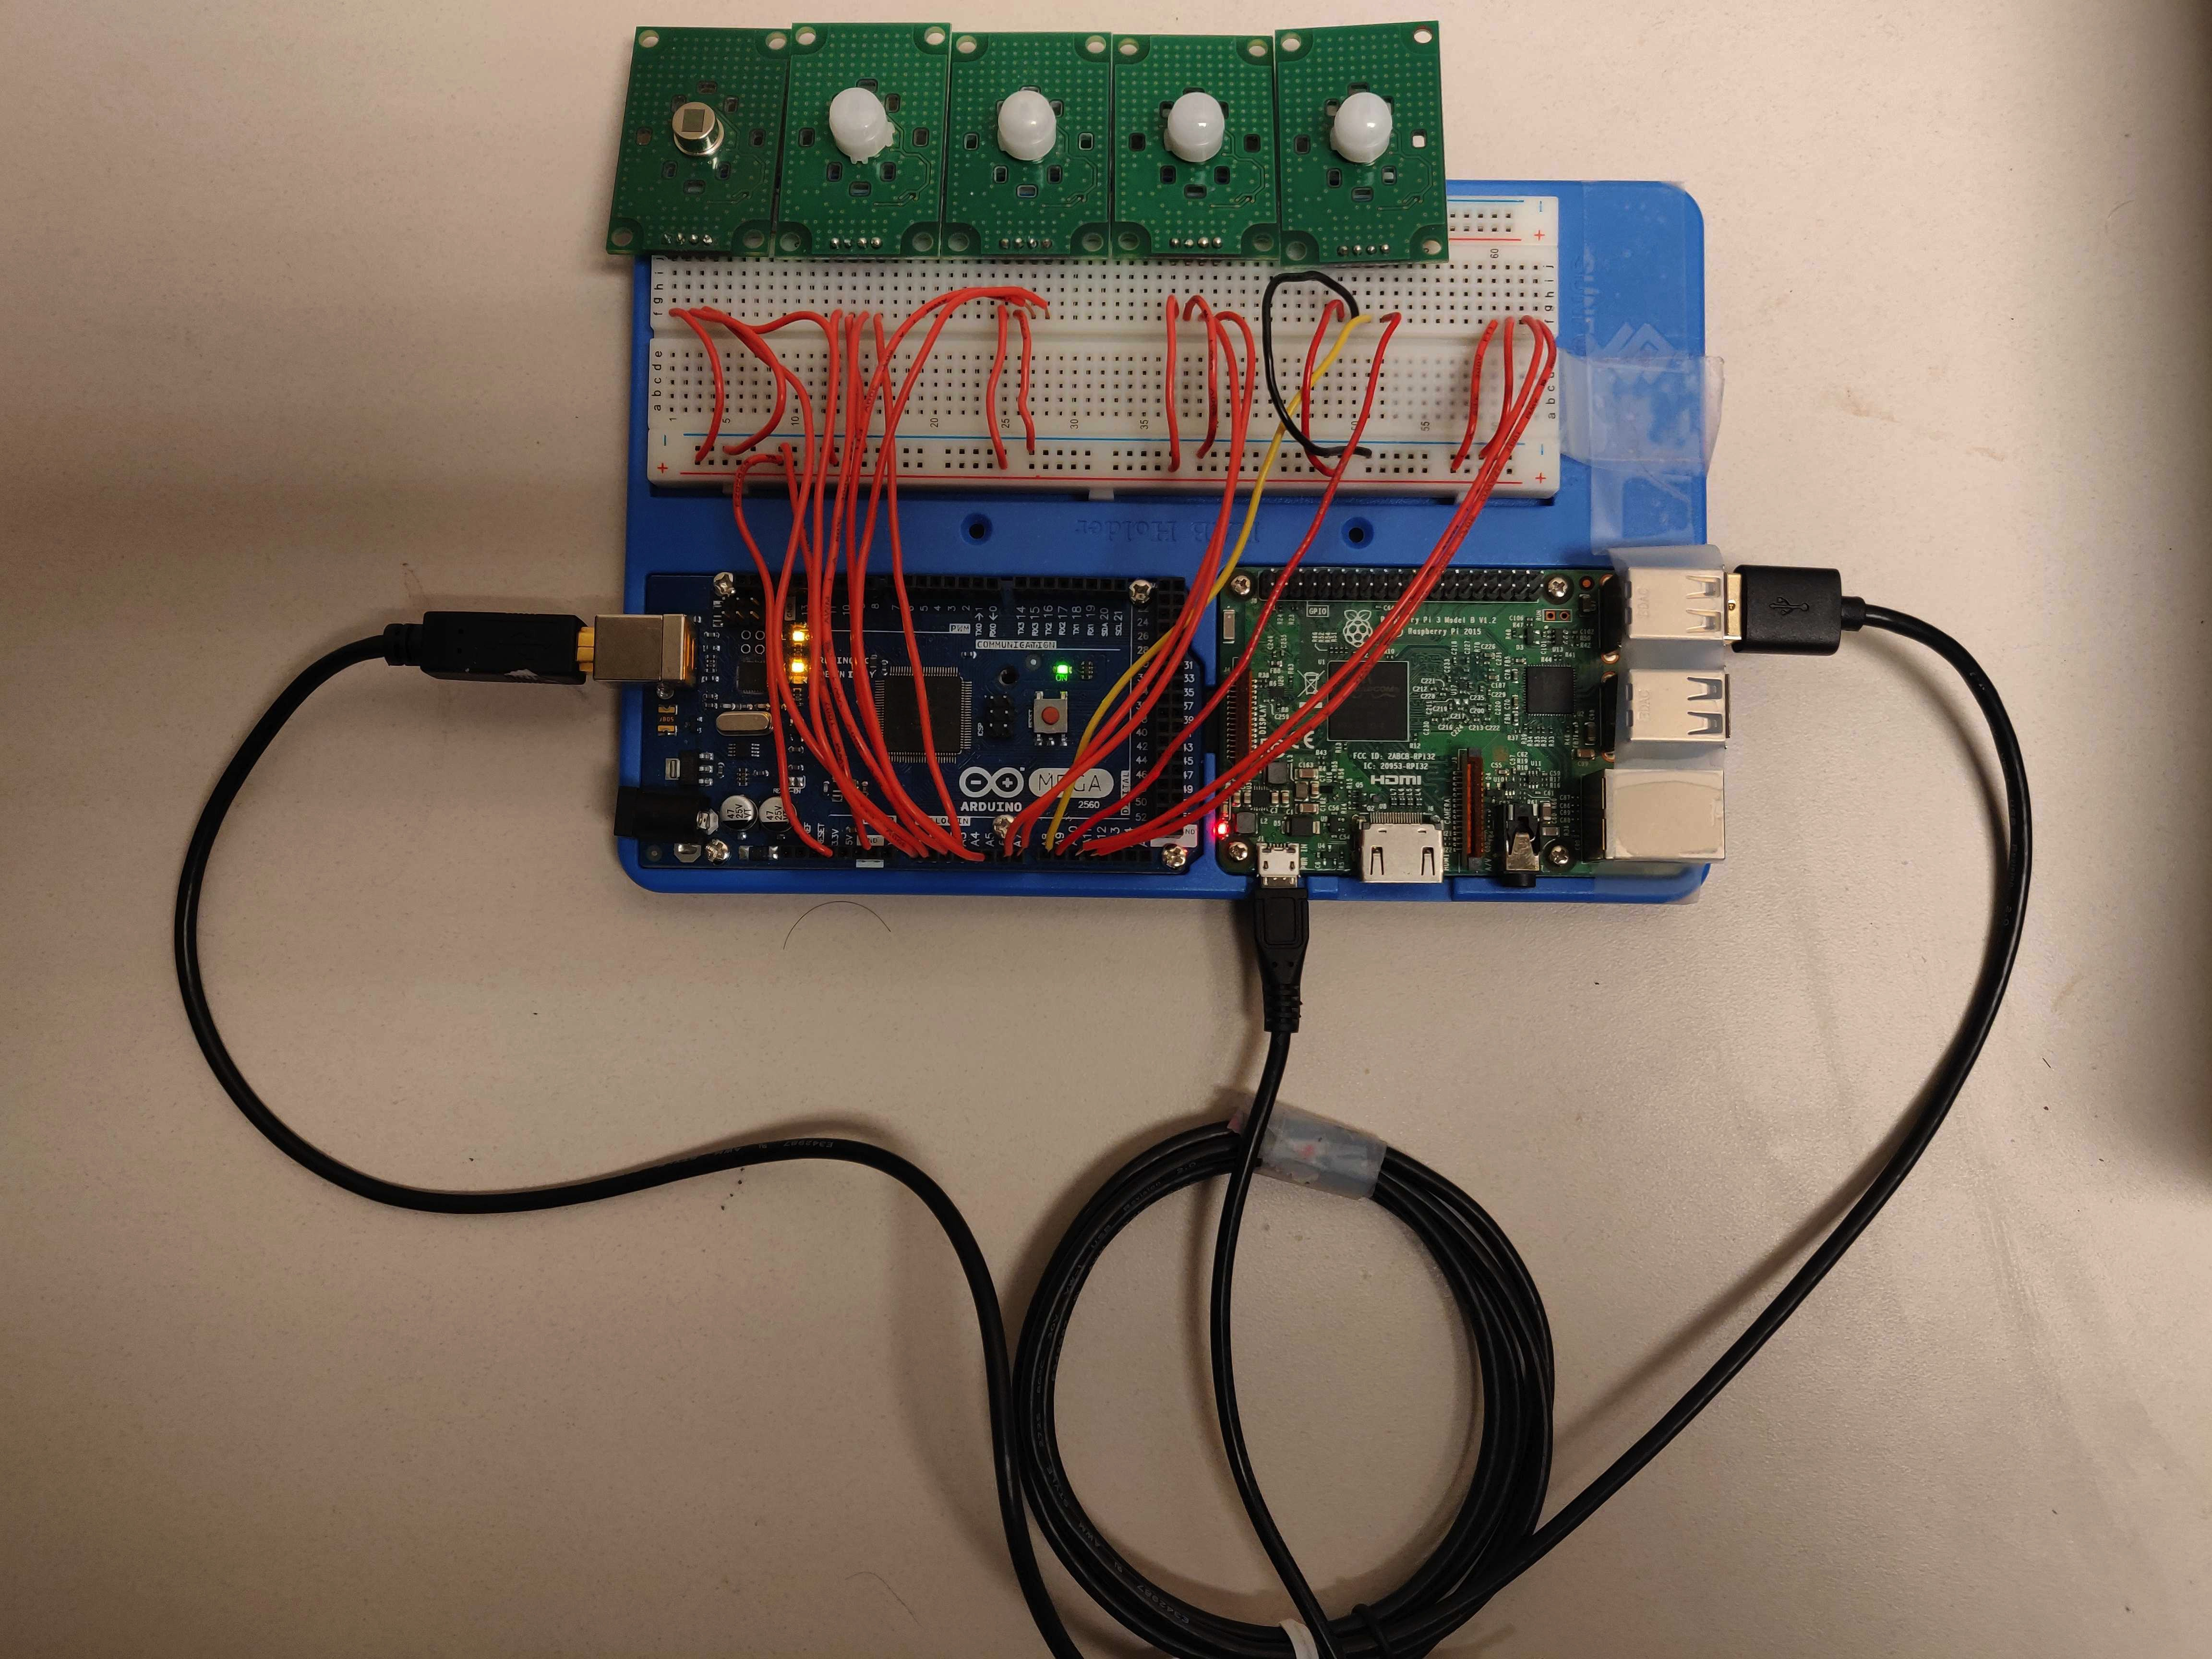
\includegraphics[width=\textwidth, height=1.2in]{figures/platform/eval_platform.jpg}
    	\captionof{figure}{Evaluation Platform showing PIR sensor connected to Raspberry Pi and Arduino.}
    	\label{fig:eval_platform}
    \end{minipage}
\end{figure}

%
%, showing capture of \aout and \cout $\rightarrow$ feature extraction $\rightarrow$ fault classification $\rightarrow$ fault identification is illustrated in {\bfseries Fig.~\ref{fig:system_workflow}}.
%
% and a photograph of our platform is shown in Fig~\ref{fig:platform_photograph}. 


% \cc \textbf{Data Cleaning and Pre-processing} %We use the \aout waveform captured from the PIR sensor and extract features by characterising it both in the frequency and time domain. We split the signal into time windows of 1024 samples. %Window sizes are typically powers of 2, as standard FFT implementations use radix-2 algorithms. 
% We shift the \aout output signal to make it zero-mean by subtracting the mean and for the FFT feature, we normalize the FFT by the window size (1024) to remove scaling effects.% caused by the window size.

%Our anonymized implementation with collected data is available at \url{https://anonymous.4open.science/r/b63479fd-8357-46d9-a776-b4a3356bef5c/}.

%The fourier coefficients obtained are used to train a supervised machine learning model and for the purposes of classification and identification, we use a standard Random Forest classifier. 
\subsection{Parameters of \sol}
\label{subsec:prac} 
\ci \textbf{Size of Window}: The collected \aout waveform is split into equal-size sample windows over which features are calculated. We observed that using a window too small (\eg 128) does not allow us to capture sufficient features for a failure type and could lead to a large number of false alarms. Also, too large of a window size (\eg 8192) leads to an overlap in the features of multiple failure classes leading to a loss of accuracy. The variation of model accuracy as a function of window size is shown in {\bfseries Fig.~\ref{fig:accuracy_vs_window_size}}. We chose a window size of 1024 samples 
%\sout{for our purpose. Using a window size of 1024 samples} 
as it gave us a good trade-off between time to capture a window (approx. 50 seconds) and accuracy (> 98\%).

\cii \textbf{Benjamini-Hochberg (B-H) Feature Selection} While there are more than 300 features that can be derived for time series analysis of \aout, B-H feature selection process (derived from parameterized hypothesis testing)~\cite{benjamini1995controlling,christ2018time} prunes this to a lower number of features that can sufficiently capture the physics of the system. We observed that using more than 10 features did not contribute to a significant increase in accuracy (beyond 98\%) and can, in practice, lead to lower performance due to overfitting as described in \S\ref{subsec:bh}.%\sout{To reduce the number of features collected and to extract important features, we use the B-H feature selection process. A lower number of features reduces accuracy of the model and a higher number of features increases amount of compute resources needed and can also lead to poor performance due to overfitting.} 
%We found that in practice the desired accuracy was achieved using around 10 features, which are derivatives of time and frequency domain representations of \aout.

\ciii \textbf{Classifier Model}: We used a Random Forest classifier~\cite{polikar2012ensemble, breiman2001random} owing to the capability to classify data based on ``entropy'' or the information gain.  % Our purpose of a classifier is to capture the information presented in K-S statistic (\S\ref{subsec:learnability}). 
Random Forest uses an ensemble of trees and has been shown to give high predictive accuracy and control over-fitting in practice, both of which are issues with decision trees. Additionally, Random Forests are amenable to interpretation by techniques such as Shapley TreeExplainer~\cite{lundberg2020local2global} that explains the features influencing prediction. \textit{Finally, we note that \aout is compatible with any classification algorithm.}

%\ashish{Random Forest Classifier analysis needs to be brought upfront - make it a subsection of its own. This process uses an ensemble of decision trees and analyzes how each feature affects the decisions across all the trees. We pass a decision tree trained offline using our training data into the Shapley TreeExplainer~\cite{lundberg2020local2global} which explains the the features influencing the prediction of the desicison tree.}


%Random Forest~\cite{polikar2012ensemble, breiman2001random} is a classification algorithm used to identify which group an observation belongs to. Random Forest is an collection of uncorrelated decision trees, each of which are trained on a random subset of the dataset. This produces a forest that operate on a whole to be greater than any of the individual constituent trees -- an effect in machine learning called ensemble learning. There are many other classification algorithms in the domain of data science~\eg Logistic Regression, Support Vector Machine, Naive Bayes Classifier and Decision Trees. 

%We note that the use of \aout is independent of the ML algorithm used and other ML algorithms such as kNN can also be eaily used here.

% random forest classifier~\cite{breiman2001random} that uses entropy (\ie information gain) to classify the sensors in working and faulty, with the class of fault as applicable.
